%%%_* Document preamble
\documentclass[14pt,t,usepdftitle=false,xcolornames=x11names,svgnames,dvipsnames,usenames]{beamer}
% \usepackage[T1]{fontenc}
\usepackage{fontspec}
\usepackage{listings}
\usepackage{alltt}

\input{texsrc/haskell.sty}
%%%_* Simplest theme ever; white background, no widgets
\newcommand{\lmss}{\fontfamily{lmtt}\selectfont\small}
\newcommand{\mlmss}{\fontfamily{lmtt}\selectfont\footnotesize}
\newcommand{\slmss}{\fontfamily{lmtt}\selectfont\scriptsize}
\usetheme{default}
\setbeamertemplate{navigation symbols}{}
\setbeameroption{show notes}
\setbeamertemplate{frametitle}[default][center]
\setbeamersize{text margin left=10mm}
%%%_** Fancy fonts
\setbeamerfont{frametitle}{}
\setmainfont[Mapping=tex-text]{Latin Modern Sans}
\setsansfont[Mapping=tex-text,Numbers={OldStyle}]{Latin Modern Sans}
\setmonofont[Mapping=tex-text]{Latin Modern Mono}
\newcommand{\wackyFont}[1]{
  {\LARGE\fontspec[Mapping=tex-text]{Trebuchet MS} #1}}
\newcommand{\includelisting}[1]{
  {\lmss\input{#1}}}
\newcommand{\sincludelisting}[1]{
  {\slmss\input{#1}}}
\newcommand{\mincludelisting}[1]{
  {\mlmss\input{#1}}}
\newcommand{\subtitleFont}[1]{{\footnotesize #1}}
\newcommand{\slideheading}[1]{
  \begin{center}
    \usebeamerfont{frametitle}
    \usebeamercolor[fg]{frametitle}#1
  \end{center}\vskip-5mm}
\usefonttheme{professionalfonts}
%%%_** Color definitions
\colorlet{comment}{Olive}
\colorlet{string}{SaddleBrown}
\colorlet{keyword}{Navy}
\colorlet{type}{Green}
\colorlet{emph}{Maroon}
\colorlet{input}{Indigo}
\colorlet{error}{DarkRed}
\colorlet{result}{LightSlateGrey}
\colorlet{background}{LightGoldenrodYellow}
\colorlet{hole}{LimeGreen}

%%%_* Metadata
\title{\wackyFont{Applicative Functors}}
\subtitle{\textbf{Hidden in plain view...}}
\author{Jim~Powers\\\subtitleFont{Patch.com}}
\date{\subtitleFont{NYC Functional Programming Meetup\\25 October 2011}}
%%%_* Document
\begin{document}

\lstset{
  language=Haskell,
  columns=flexible,
  showstringspaces=false,
  basicstyle={\small\ttfamily},
  keywordstyle={\bfseries\color{keyword}},
  commentstyle=\color{comment},
  stringstyle=\color{string},
  emphstyle={\color{type}},
  emphstyle={[2]\color{emph}},
  breakatwhitespace=true,
  tabsize=2
}

\maketitle

\section{Inspiration}

\begin{frame}{Inspiration}
  \sincludelisting{texsrc/ApplicBuildName.hs.tex}\\
  \uncover<2->{Won't compile:\\\sincludelisting{texsrc/ApplicDesired.hs.tex}\\}
  \uncover<3->{Not bad:\\\sincludelisting{texsrc/ApplicNice.hs.tex}}
\end{frame}

\begin{frame}{Inspiration}
  \begin{center}
    
\includegraphics[scale=.7]{images/Applicative.png}
  \end{center}
\end{frame}

\begin{frame}{Inspiration}
  \vskip+20mm
  \begin{itemize}[<+->]
    \item{Applicative?}
    \item{Functors?}
    \item{Effects?}
  \end{itemize}
\end{frame}

\section{Orienting ourselves}

\begin{frame}{Family Tree}
  \vspace{-7mm}
  \begin{center}
    \includegraphics[scale=.42]{dotpdf/dependencies.pdf}\\
    \tiny{\emph{Typeclassopedia}, Brent Yorgey, TMR-issue13}
  \end{center}
\end{frame}

\begin{frame}{Family Tree}
  \vspace{-7mm}
  \begin{center}
    \includegraphics[scale=.42]{dotpdf/dependencies-applicative.pdf}\\
    \tiny{\emph{Typeclassopedia}, Brent Yorgey, TMR-issue13}
  \end{center}
\end{frame}

\section{Functor}

\begin{frame}{Functor}
  \includelisting{texsrc/Functor.hs.tex}
\end{frame}

\begin{frame}{Functor}
  \includelisting{texsrc/Functor.hs.tex}
  \hrulefill\\
  \textbf{Functors} enable performing a computation within a context.  The function does not know anything about the context it is running in.
\end{frame}

\begin{frame}{Functor}
  \includelisting{texsrc/Functor.hs.tex}
  \hrulefill
  \begin{center}
  Functor Laws
  \end{center}
  \includelisting{texsrc/FunctorLaws.hs.tex}
\end{frame}

\begin{frame}{Functor}
  \includelisting{texsrc/Functor.hs.tex}
  \hrulefill
  \begin{center}
  Common Functor Instances
  \end{center}
  \sincludelisting{texsrc/CFI1.hs.tex}
  \uncover<2->{
  \begin{center}
  Example
  \end{center}
  \sincludelisting{texsrc/CFI1ex.hs.tex}}
\end{frame}

\begin{frame}{Functor}
  \includelisting{texsrc/Functor.hs.tex}
  \hrulefill
  \begin{center}
  Common Functor Instances
  \end{center}
  \sincludelisting{texsrc/CFI2.hs.tex}
  \uncover<2->{
  \begin{center}
  Example
  \end{center}
  \sincludelisting{texsrc/CFI2ex.hs.tex}}
\end{frame}

\begin{frame}{Functor}
  \includelisting{texsrc/Functor.hs.tex}
  \hrulefill
  \begin{center}
  Common Functor Instances
  \end{center}
  \sincludelisting{texsrc/CFI3.hs.tex}
  \uncover<2->{
  \begin{center}
  Example
  \end{center}
  \sincludelisting{texsrc/CFI3ex.hs.tex}}
\end{frame}

\begin{frame}{Functor}
  \includelisting{texsrc/Functor.hs.tex}
  \hrulefill
  \begin{center}
  Common Functor Instances
  \end{center}
  \sincludelisting{texsrc/CFI4.hs.tex}
  \uncover<2->{
  \begin{center}
  Example
  \end{center}
  \sincludelisting{texsrc/CFI4ex.hs.tex}}
\end{frame}

\section{Pointed}

\begin{frame}{Pointed}
\includelisting{texsrc/Pointed.hs.tex}
\end{frame}

\begin{frame}{Pointed}
  \includelisting{texsrc/Pointed.hs.tex}
  \hrulefill\\
  The \textbf{Pointed} typeclass is not represented in the Haskell standard library by itself.  Conceptually, \textbf{Pointed} presents the ability to \textbf{lift} an ordinary value into a context, thus creating a \textbf{point} in that context.
\end{frame}

\section{Applicative}

\begin{frame}{Applicative}
\includelisting{texsrc/Applicative.hs.tex}
\end{frame}

\begin{frame}{Applicative}
\includelisting{texsrc/Applicative.hs.tex}
  \hrulefill\\
  The \textbf{Applicative} combines that ability to create a \textbf{point} within a context, as well as the ability to apply a \textbf{lifted} function within that context.\\
  \vskip+5mm\uncover<2->{Each context expresses how to apply the lifted function in its own particular way.  Also known as its \textbf{idiom}.}
\end{frame}

\begin{frame}{Applicative}
  \includelisting{texsrc/Applicative.hs.tex}
  \hrulefill
  \begin{center}
  Applicative Laws
  \end{center}
  \includelisting{texsrc/ApplicativeLaws.hs.tex}
\end{frame}

\begin{frame}{Applicative}
  \includelisting{texsrc/Applicative.hs.tex}
  \hrulefill
  \begin{center}
  Common Applicative Instances
  \end{center}
  \sincludelisting{texsrc/CAI1.hs.tex}
  \uncover<2->{
  \begin{center}
  Example
  \end{center}
  \sincludelisting{texsrc/CAI1ex.hs.tex}}
\end{frame}

\begin{frame}{Applicative}
  \includelisting{texsrc/Applicative.hs.tex}
  \hrulefill
  \begin{center}
  Common Applicative Instances
  \end{center}
  \sincludelisting{texsrc/CAI2.hs.tex}
  \uncover<2->{
  \begin{center}
  Example
  \end{center}
  \sincludelisting{texsrc/CAI2ex.hs.tex}}
\end{frame}

\begin{frame}{Applicative}
  \includelisting{texsrc/Applicative.hs.tex}
  \hrulefill
  \begin{center}
  Common Applicative Instances
  \end{center}
  \sincludelisting{texsrc/CAI3.hs.tex}
  \uncover<2->{
  \begin{center}
  Example
  \end{center}
  \sincludelisting{texsrc/CAI3ex.hs.tex}}
\end{frame}

\begin{frame}{Applicative}
  \includelisting{texsrc/Applicative.hs.tex}
  \hrulefill
  \begin{center}
  Common Applicative Instances
  \end{center}
  \sincludelisting{texsrc/CAI4.hs.tex}
  \uncover<2->{
  \begin{center}
  Example
  \end{center}
  \sincludelisting{texsrc/CAI4ex.hs.tex}}
\end{frame}

\begin{frame}{Inspiration}
  \sincludelisting{texsrc/ApplicBuildName.hs.tex}\\
  Won't compile:\\\sincludelisting{texsrc/ApplicDesired.hs.tex}\\
  Not bad:\\\sincludelisting{texsrc/ApplicNice.hs.tex}\\
  \uncover<2->{Sweet:\\\sincludelisting{texsrc/ApplicSweet.hs.tex}}
\end{frame}

\begin{frame}{Applicative}
\includelisting{texsrc/Applicative.hs.tex}
  \hrulefill\\
  \textbf{Applicatives} can be used as a tool to remove boilerplate!\\
  \uncover<2->{\vskip+5mm\begin{center}
  Orly? How?
  \end{center}}
\end{frame}

\begin{frame}{Applicative}
\includelisting{texsrc/Applicative.hs.tex}
  \hrulefill\\
  Predictable web example!
\end{frame}

\begin{frame}{Family Tree}
  \vspace{-7mm}
  \begin{center}
    \includegraphics[scale=.42]{dotpdf/dependencies-applicative.pdf}\\
    \tiny{\emph{Typeclassopedia}, Brent Yorgey, TMR-issue13}
  \end{center}
\end{frame}

\begin{frame}{Family Tree}
  \vspace{-7mm}
  \begin{center}
    \includegraphics[scale=.42]{dotpdf/dependencies-monad.pdf}\\
    \tiny{\emph{Typeclassopedia}, Brent Yorgey, TMR-issue13}
  \end{center}
\end{frame}

\begin{frame}{Mo'nads!}
  \vspace{-7mm}
  \begin{center}
    
\includegraphics[scale=.42]{images/monads.jpg}\\
    \tiny{http://twitpic.com/5j3x2t}
  \end{center}
\end{frame}

\begin{frame}{Web Example}
\sincludelisting{texsrc/Request.hs.tex}
\end{frame}

\begin{frame}{Web Example}
\sincludelisting{texsrc/Response.hs.tex}
\end{frame}

\begin{frame}{Web Example}
\begin{center}
  Reader Monad
\end{center}
\sincludelisting{texsrc/Reader.hs.tex}
\hrulefill\\
\sincludelisting{texsrc/RequestReader.hs.tex}
\end{frame}

\begin{frame}{Web Example}
\sincludelisting{texsrc/MaybeResult.hs.tex}
\end{frame}

\begin{frame}{Web Example}
\sincludelisting{texsrc/MonadReader.hs.tex}
\end{frame}

\begin{frame}{Web Example}
\sincludelisting{texsrc/MonadReaderRun.hs.tex}
\end{frame}

\begin{frame}{Web Example}
\sincludelisting{texsrc/MonadReaderRun.hs.tex}
\begin{itemize}[<+->]
  \item => \footnotesize{``Page rendered STRING: James Powers''}
  \item => \footnotesize{``BZZT! Invalid request: [Required value for:last missing]''}
  \item => \footnotesize{``BZZT! Invalid request: [Required value for:first missing]''}
  \item => Hrm...
\end{itemize}
\end{frame}

\begin{frame}{Web Example}
\sincludelisting{texsrc/MaybeResultApplicative.hs.tex}
\end{frame}

\begin{frame}{Web Example}
\sincludelisting{texsrc/ApplicativeHandler.hs.tex}
\end{frame}

\begin{frame}{Web Example}
\sincludelisting{texsrc/MonadReaderRun.hs.tex}
\begin{itemize}[<+->]
  \item => \footnotesize{``Page rendered STRING: James Powers''}
  \item => \footnotesize{``BZZT! Invalid request: [Required value for:last missing]''}
  \item => \footnotesize{``BZZT! Invalid request: [Required value for:first missing,Required value for:last missing]''}
  \item => Whoa!  Now dats powah!
\end{itemize}
\end{frame}

\begin{frame}{Applicatives vs. Monads}
\begin{itemize}[<+->]
  \item Monads enable \textbf{conditional} (short-circuited) computation.
  \item Monads can be \textbf{stacked} through \textbf{monad transformers}.
  \item Monads are much more restrictive and hence less common.
\end{itemize}
\end{frame}

\begin{frame}{Family Tree}
  \vspace{-7mm}
  \begin{center}
    \includegraphics[scale=.42]{dotpdf/dependencies-monad.pdf}\\
    \tiny{\emph{Typeclassopedia}, Brent Yorgey, TMR-issue13}
  \end{center}
\end{frame}

\begin{frame}{Family Tree}
  \vspace{-7mm}
  \begin{center}
    \includegraphics[scale=.42]{dotpdf/dependencies-traversable.pdf}\\
    \tiny{\emph{Typeclassopedia}, Brent Yorgey, TMR-issue13}
  \end{center}
\end{frame}

\begin{frame}{Monoid}
  \includelisting{texsrc/Monoid.hs.tex}
\end{frame}

\begin{frame}{Foldable}
  \includelisting{texsrc/Foldable.hs.tex}
\end{frame}

\begin{frame}{Must Read!}
  \begin{center}
    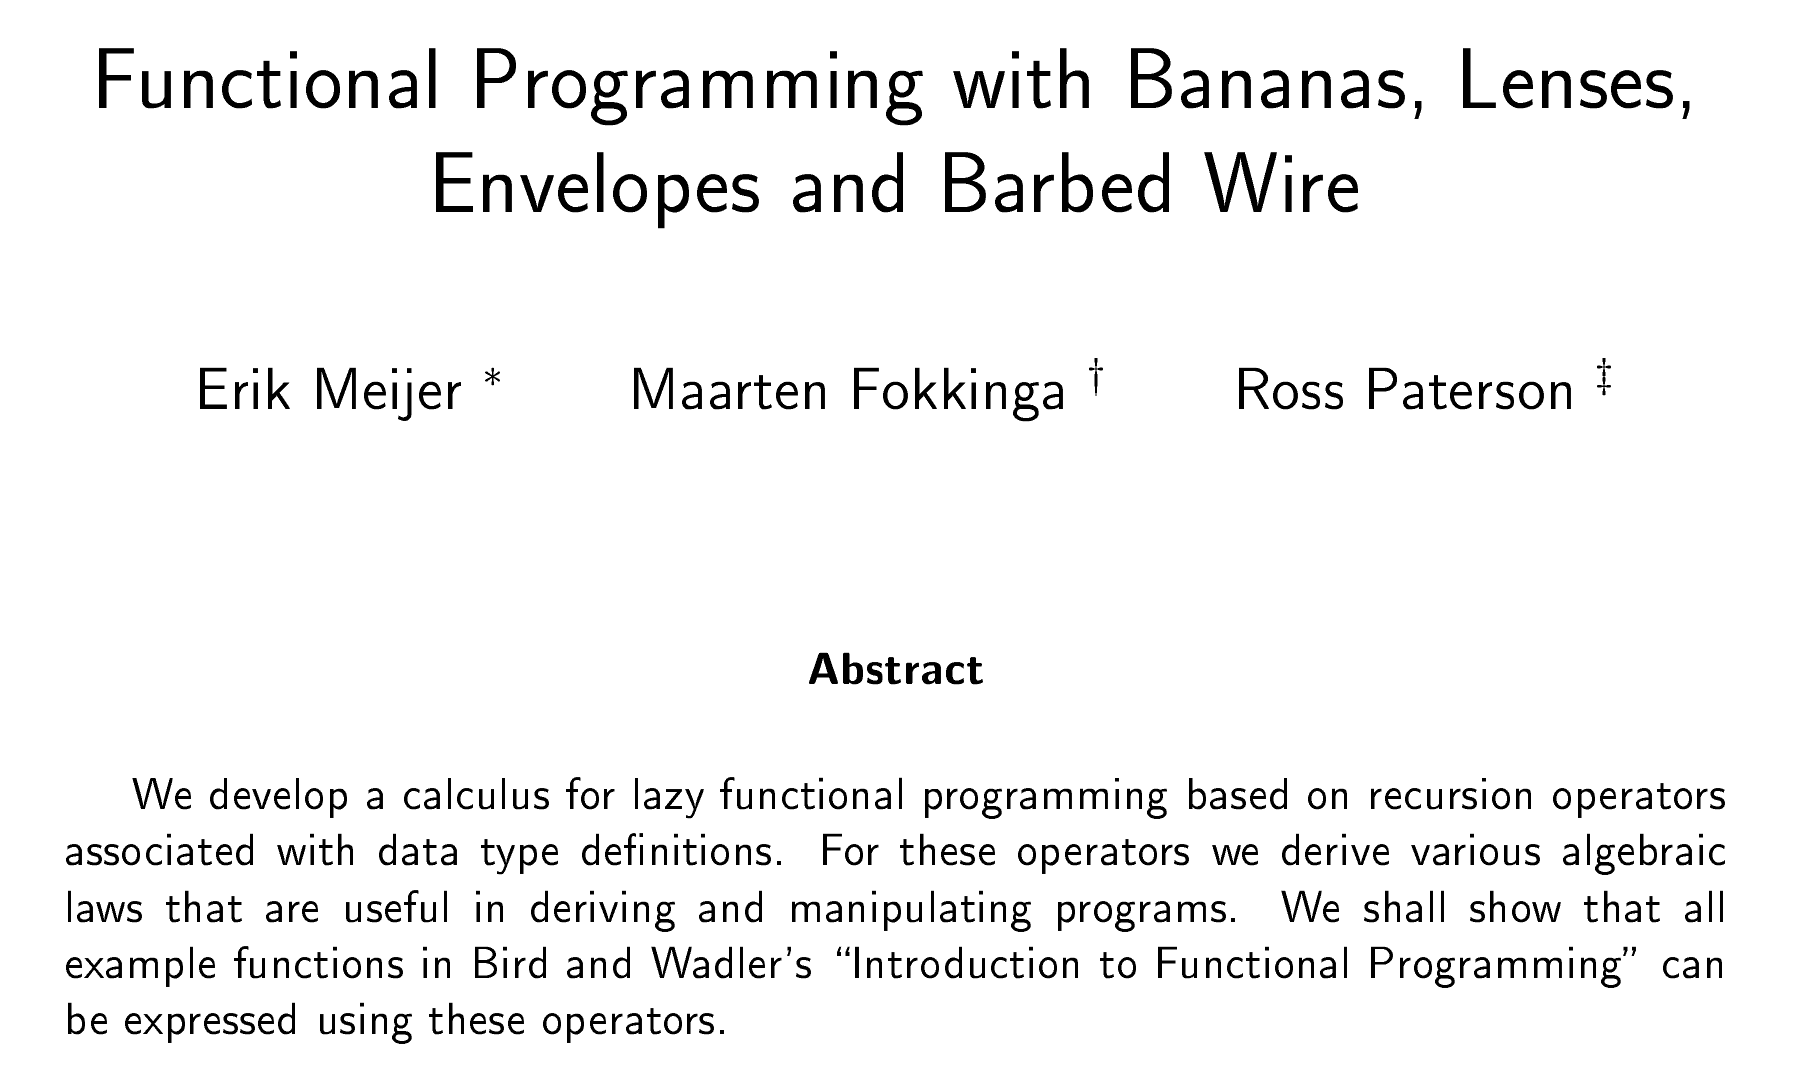
\includegraphics[scale=.7]{images/Catamorphisms.png}
  \end{center}
\end{frame}

\begin{frame}{All sorts of folds...}
\begin{itemize}[<+->]
  \item Anamorphism
  \item Apomorphism
  \item Hylomorphism
  \item Paramorphism
\end{itemize}
\end{frame}

\begin{frame}{Must Read!}
  \begin{center}
    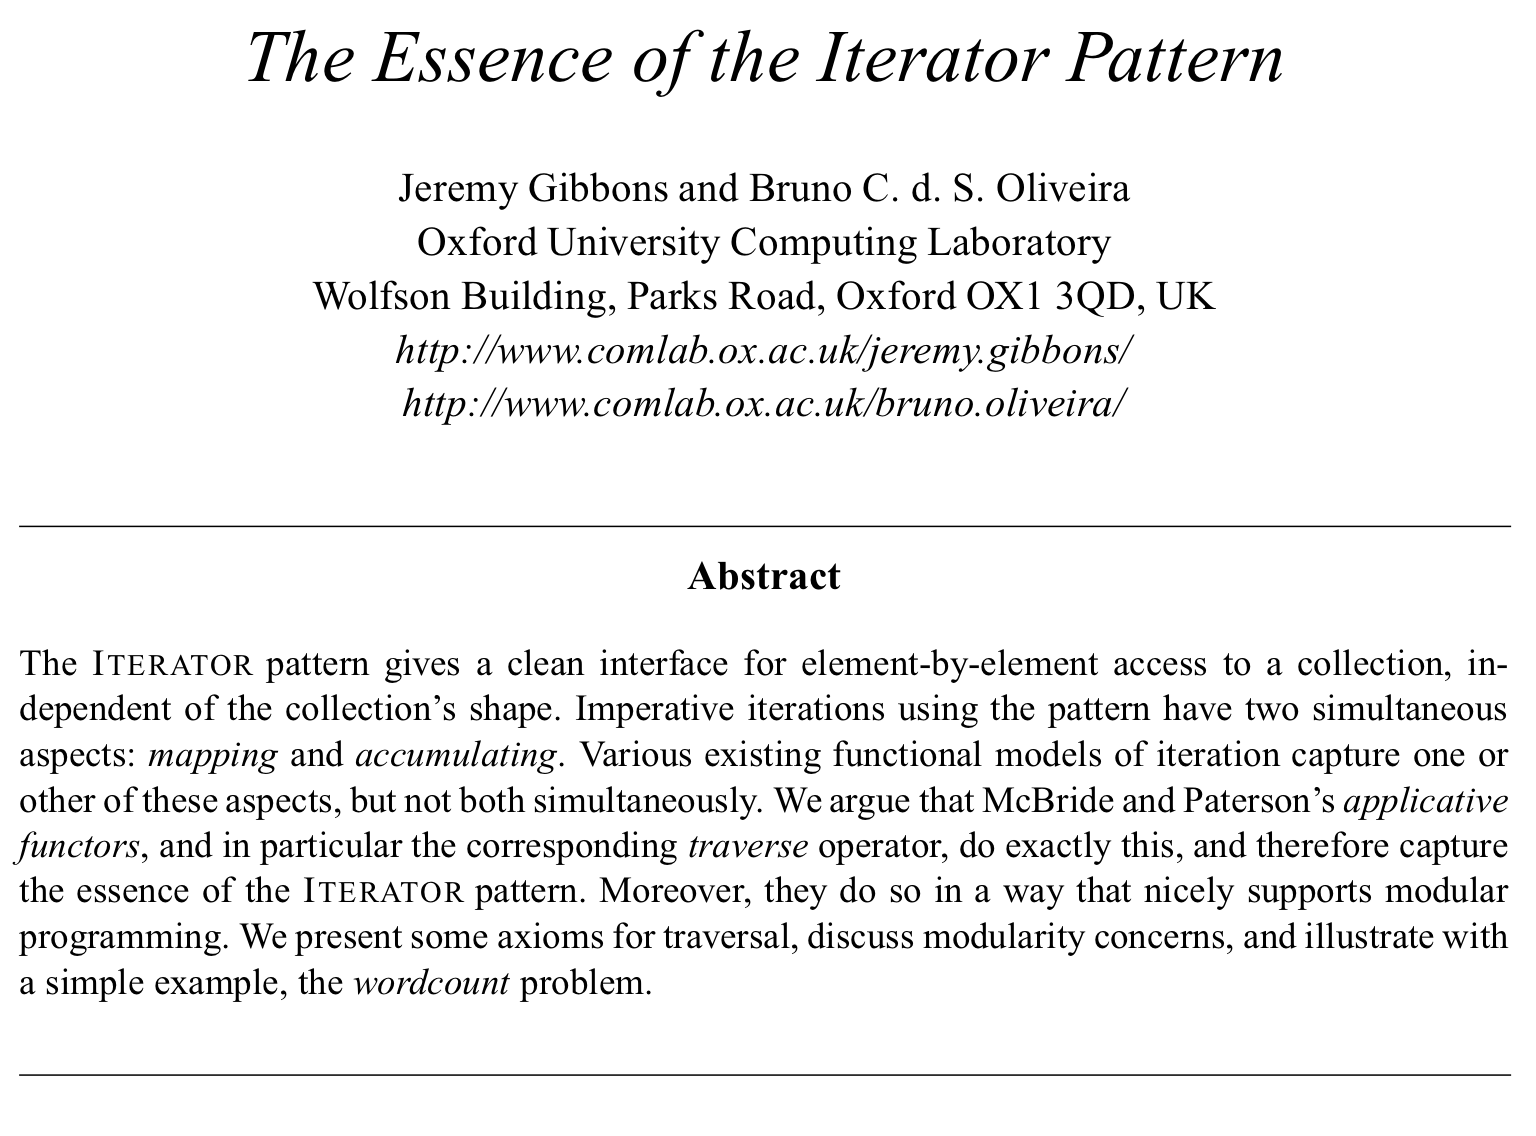
\includegraphics[scale=.7]{images/Iterator.png}
  \end{center}
\end{frame}

\begin{frame}{Traversable}
  \sincludelisting{texsrc/Traversable.hs.tex}\\
  \uncover<2->{\hrulefill\\\includelisting{texsrc/TraversableSuccess.hs.tex}\\
  \small{=> Just [1,2]}\\}
  \uncover<3->{\hrulefill\\\includelisting{texsrc/TraversableFail.hs.tex}\\
  \small{=> Nothing}}
\end{frame}

\end{document}